\documentclass[a4paper]{article}

\usepackage[utf8]{inputenc}
\usepackage[T1]{fontenc}
\usepackage[portuguese]{babel}
\usepackage{parskip}
\usepackage[normalem]{ulem}
\usepackage[dvipsnames]{xcolor}
\usepackage{minted}
\usepackage{graphicx}
\usepackage{float}
\usepackage{hyperref}

\definecolor{LightGray}{gray}{0.95}
\usemintedstyle{pastie}
\setminted{breaklines=true, breakanywhere=true, fontsize=\small}

\begin{document}

\title{Trabalho de Banco de Dados 1 - Praestitia}
\author{João Luis Almeida Santos}
\maketitle

\tableofcontents
\newpage

\section{Introdução}

Este trabalho apresenta o projeto de banco de dados relacional que dá suporte a
Praestitia, um sistema de CRM voltado ao gerenciamento de leads, clientes e concorrentes.
O objetivo é exercitar a passagem do modelo conceitual para o modelo lógico, sua
implementação no modelo físico em PostgreSQL e, por fim, a escrita de consultas SQL que
respondam a perguntas relevantes do negócio.

O documento está organizado em quatro partes. Primeiro, descreve-se Praestitia e o
domínio que atende. Em seguida, apresenta-se o modelo lógico com as relações e a
justificativa de cada chave estrangeira. A terceira parte exibe e explica cada uma das
consultas SQL desenvolvidas sobre o esquema. Por fim, a conclusão recapitula os pontos
principais do trabalho.

\section{Praestitia}

Praestitia é um CRM que organiza o funil comercial de uma empresa, acompanhando um
contato desde o primeiro interesse até a conversão em cliente efetivo e também registrando
os concorrentes que atuam no mesmo mercado. O sistema é multiusuário, e cada vendedor
cadastrado é responsável pelos registros que cria.

O domínio é composto pelas seguintes entidades.

\begin{itemize}
    \item \textbf{Usuário}, o vendedor que opera o sistema. É responsável pelos leads,
    clientes e concorrentes que cadastra e pertence a um grupo de permissões.
    \item \textbf{Grupo e Permissão}, que controlam a autorização. Um grupo reúne um
    conjunto de permissões e um usuário herda as permissões do seu grupo. A relação entre
    grupo e permissão é de muitos para muitos.
    \item \textbf{Lead}, contato que demonstrou interesse inicial, mas ainda não foi
    convertido. Guarda a origem do contato, o status no funil de vendas e uma pontuação
    que indica o quão promissor é o lead.
    \item \textbf{Cliente}, lead convertido ou contato que já fechou negócio. Possui um
    status comercial, que pode ser ativo, inativo, pendente ou suspenso.
    \item \textbf{Concorrente}, empresa que disputa o mesmo mercado, registrada para
    acompanhamento competitivo.
    \item \textbf{Endereço}, dados de localização reutilizáveis, referenciados por leads,
    clientes e concorrentes.
\end{itemize}

Esse domínio justifica as consultas apresentadas mais adiante. Medir a origem dos leads,
acompanhar o funil de vendas, identificar a carga de trabalho por usuário e cruzar leads
com clientes já existentes são operações típicas do dia a dia de um CRM.

\section{Modelo Conceitual}

O modelo conceitual representa o domínio de Praestitia em um diagrama
Entidade-Relacionamento, antes de qualquer preocupação com a tecnologia do banco. Ele
mostra as entidades Permissao, Grupo, Usuario, Endereco, Lead, Cliente e Concorrente, seus
atributos e os relacionamentos entre elas.

Os principais relacionamentos são os seguintes. Um Grupo reúne muitas Permissões e uma
Permissão pode estar em muitos Grupos, formando um relacionamento de muitos para muitos.
Cada Usuario pertence a um Grupo, e um Grupo pode ter muitos Usuarios. Um Usuario é
responsável por muitos Leads, Clientes e Concorrentes, e cada um desses registros pertence
a um único Usuario. Por fim, Lead, Cliente e Concorrente podem apontar para um Endereco,
que pode ser compartilhado por mais de um registro.

\begin{figure}[H]
    \centering
    \IfFileExists{modelo_conceitual.png}{%
        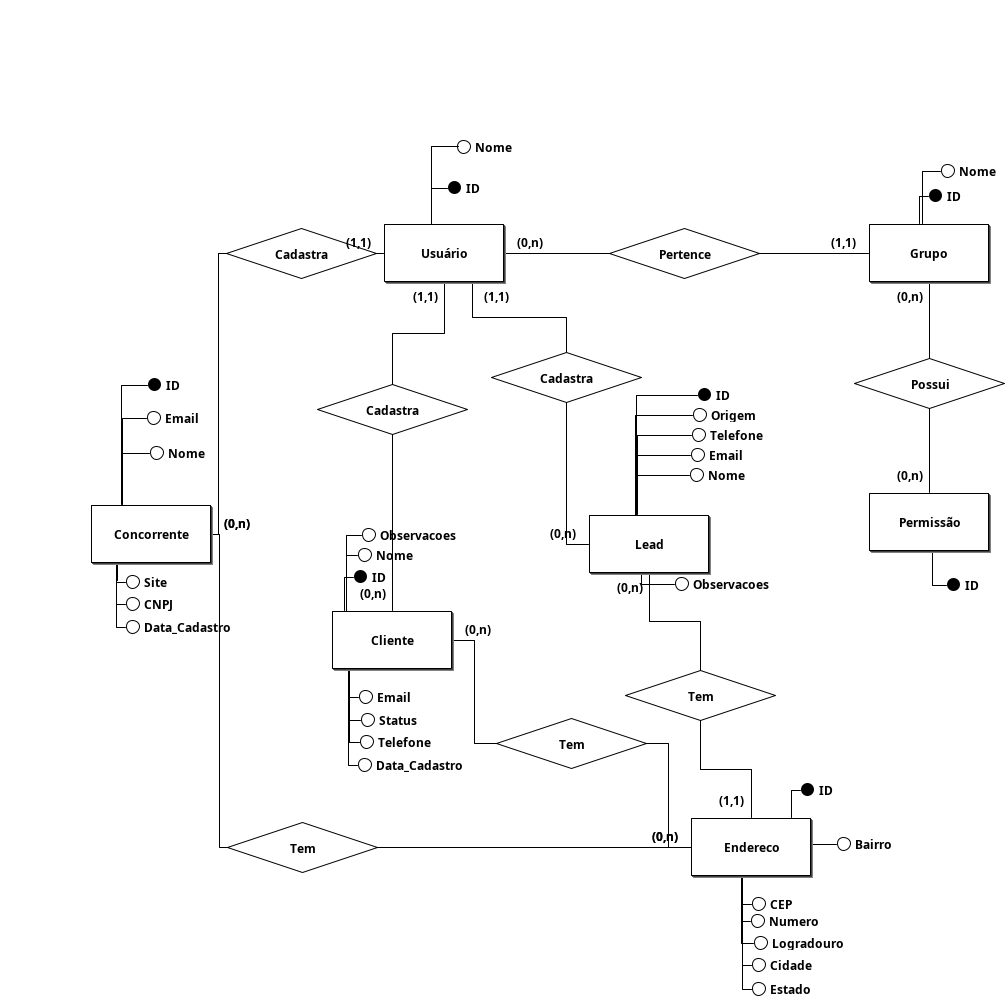
\includegraphics[width=\linewidth]{modelo_conceitual.png}%
    }{\textit{[Inserir aqui a imagem modelo\_conceitual.png exportada do brModelo.]}}
    \caption{Modelo conceitual de Praestitia (diagrama Entidade-Relacionamento).}
\end{figure}

\section{Modelo Lógico}

O modelo lógico mapeia o diagrama conceitual para o modelo relacional, transformando cada
entidade em uma tabela e cada relacionamento em chaves estrangeiras. Chave primária
sublinhada. Chave estrangeira marcada com asterisco.

\bigskip

\begingroup
\sloppy

\textbf{Permissao}(\uline{id})

\textbf{Grupo}(\uline{id}, nome)

\textbf{Grupo\_Permissao}(\uline{*grupo\_id}, \uline{*permissao\_id})

\textbf{Usuario}(\uline{id}, nome, *grupo\_id)

\textbf{Endereco}(\uline{id}, cep, numero, logradouro, bairro, cidade, estado)

\textbf{Lead}(\uline{id}, *usuario\_id, *endereco\_id, nome, email, telefone, empresa, cargo, origem, interesse, status, pontuacao, observacoes, data\_cadastro, data\_ultimo\_contato)

\textbf{Cliente}(\uline{id}, *usuario\_id, *endereco\_id, nome, email, telefone, empresa, cnpj\_cpf, status, data\_cadastro, observacoes)

\textbf{Concorrente}(\uline{id}, *usuario\_id, *endereco\_id, nome, email, site, cnpj, data\_cadastro)

\endgroup

\bigskip

\textbf{Chaves estrangeiras}

\begin{itemize}
    \item \textbf{Grupo\_Permissao.grupo\_id referencia Grupo(id).} Um grupo pode ter várias permissões e uma permissão pode estar em vários grupos ao mesmo tempo, o que torna a relação de muitos para muitos. Como nenhum dos dois lados consegue guardar essa informação sozinho, a solução é uma tabela intermediária que registra cada combinação.
    \item \textbf{Grupo\_Permissao.permissao\_id referencia Permissao(id).} Pelo mesmo motivo, a permissão também precisa estar representada na tabela intermediária.
    \item \textbf{Usuario.grupo\_id referencia Grupo(id).} Um usuário pertence a um grupo, mas um grupo pode ter vários usuários. A chave fica em Usuario porque é o lado que se repete na relação.
    \item \textbf{Lead.usuario\_id referencia Usuario(id).} Um usuário pode cadastrar vários leads, mas cada lead pertence a um único usuário. A chave fica em Lead porque é o lado que se repete.
    \item \textbf{Lead.endereco\_id referencia Endereco(id).} Pessoas do mesmo domicílio, como cônjuges, podem ser cadastradas como leads distintos mas compartilham o mesmo endereço. A chave fica em Lead para que o endereço não precise ser duplicado.
    \item \textbf{Cliente.usuario\_id referencia Usuario(id).} Um usuário gerencia vários clientes, mas cada cliente foi cadastrado por um único usuário. A chave fica em Cliente pelo mesmo motivo do Lead.
    \item \textbf{Cliente.endereco\_id referencia Endereco(id).} Clientes no mesmo endereço reaproveitam o mesmo registro. A chave fica em Cliente pelo mesmo motivo do Lead.
    \item \textbf{Concorrente.usuario\_id referencia Usuario(id).} Um usuário pode monitorar vários concorrentes. A chave fica em Concorrente pelo mesmo motivo dos casos anteriores.
    \item \textbf{Concorrente.endereco\_id referencia Endereco(id).} Empresas concorrentes podem estar no mesmo endereço, como num edifício comercial. A chave fica em Concorrente pelo mesmo motivo do Lead e do Cliente.
\end{itemize}

\section{Modelo Físico}

O modelo físico traduz o modelo lógico no script DDL que cria as tabelas no PostgreSQL.
Aqui são definidos os tipos de cada coluna, as chaves primárias e estrangeiras, e as
restrições de integridade que garantem a consistência dos dados.

\begin{minted}[bgcolor=LightGray]{sql}
CREATE TABLE permissao (
    id   SERIAL PRIMARY KEY
);

CREATE TABLE grupo (
    id   SERIAL       PRIMARY KEY,
    nome VARCHAR(150) NOT NULL UNIQUE
);

CREATE TABLE grupo_permissao (
    grupo_id     INTEGER NOT NULL REFERENCES grupo(id) ON DELETE CASCADE,
    permissao_id INTEGER NOT NULL REFERENCES permissao(id) ON DELETE CASCADE,
    PRIMARY KEY (grupo_id, permissao_id)
);

CREATE TABLE usuario (
    id       BIGSERIAL    PRIMARY KEY,
    nome     VARCHAR(150) NOT NULL,
    grupo_id INTEGER      REFERENCES grupo(id) ON DELETE SET NULL
);

CREATE TABLE endereco (
    id          SERIAL       PRIMARY KEY,
    cep         VARCHAR(10),
    numero      VARCHAR(20),
    logradouro  VARCHAR(200),
    bairro      VARCHAR(100),
    cidade      VARCHAR(100),
    estado      CHAR(2)
);
\end{minted}

As tabelas de leads, clientes e concorrentes guardam os contatos do funil. Note as
restrições \texttt{CHECK}, que limitam \texttt{status} e \texttt{origem} a um conjunto fixo
de valores, e o \texttt{UNIQUE} no e-mail do cliente, que impede cadastros duplicados.

\begin{minted}[bgcolor=LightGray]{sql}
CREATE TABLE lead (
    id                  SERIAL       PRIMARY KEY,
    usuario_id          BIGINT       REFERENCES usuario(id) ON DELETE CASCADE,
    endereco_id         INTEGER      REFERENCES endereco(id) ON DELETE SET NULL,
    nome                VARCHAR(200) NOT NULL,
    email               VARCHAR(254) NOT NULL,
    telefone            VARCHAR(20),
    empresa             VARCHAR(200),
    cargo               VARCHAR(100),
    origem              VARCHAR(20)  NOT NULL DEFAULT 'site',
    interesse           VARCHAR(200),
    status              VARCHAR(20)  NOT NULL DEFAULT 'novo',
    pontuacao           INTEGER      NOT NULL DEFAULT 0,
    observacoes         TEXT,
    data_cadastro       TIMESTAMPTZ  NOT NULL DEFAULT NOW(),
    data_ultimo_contato TIMESTAMPTZ,

    CONSTRAINT lead_status_check CHECK (
        status IN ('novo', 'contatado', 'qualificado', 'em_negociacao', 'convertido', 'perdido')
    ),
    CONSTRAINT lead_origem_check CHECK (
        origem IN ('site', 'indicacao', 'redes_sociais', 'email', 'telefone', 'evento', 'outro')
    )
);

CREATE TABLE cliente (
    id             SERIAL       PRIMARY KEY,
    usuario_id     BIGINT       REFERENCES usuario(id) ON DELETE CASCADE,
    endereco_id    INTEGER      REFERENCES endereco(id) ON DELETE SET NULL,
    nome           VARCHAR(200) NOT NULL,
    email          VARCHAR(254) NOT NULL UNIQUE,
    telefone       VARCHAR(20),
    empresa        VARCHAR(200),
    cnpj_cpf       VARCHAR(18),
    status         VARCHAR(20)  NOT NULL DEFAULT 'ativo',
    data_cadastro  TIMESTAMPTZ  NOT NULL DEFAULT NOW(),
    observacoes    TEXT,

    CONSTRAINT cliente_status_check CHECK (
        status IN ('ativo', 'inativo', 'pendente', 'suspenso')
    )
);

CREATE TABLE concorrente (
    id             SERIAL       PRIMARY KEY,
    usuario_id     BIGINT       NOT NULL REFERENCES usuario(id) ON DELETE CASCADE,
    endereco_id    INTEGER      REFERENCES endereco(id) ON DELETE SET NULL,
    nome           VARCHAR(200) NOT NULL,
    email          VARCHAR(254),
    site           VARCHAR(200),
    cnpj           VARCHAR(18),
    data_cadastro  TIMESTAMPTZ  NOT NULL DEFAULT NOW()
);
\end{minted}

As ações \texttt{ON DELETE} definem o que acontece com os registros dependentes quando o
registro referenciado é removido. O \texttt{ON DELETE CASCADE} em \texttt{usuario\_id}
apaga os leads, clientes e concorrentes do usuário removido, enquanto o
\texttt{ON DELETE SET NULL} em \texttt{endereco\_id} apenas desfaz o vínculo, preservando o
registro sem o endereço.

\subsection{Eficiência}

Para acelerar as consultas mais frequentes, o modelo físico cria índices sobre as colunas
usadas em filtros e junções. Sem índice, o banco precisa varrer a tabela inteira; com
índice, ele localiza as linhas diretamente.

\begin{minted}[bgcolor=LightGray]{sql}
CREATE INDEX idx_usuario_grupo       ON usuario(grupo_id);
CREATE INDEX idx_lead_usuario        ON lead(usuario_id);
CREATE INDEX idx_lead_email          ON lead(email);
CREATE INDEX idx_cliente_usuario     ON cliente(usuario_id);
CREATE INDEX idx_cliente_email       ON cliente(email);
CREATE INDEX idx_cliente_status      ON cliente(status);
CREATE INDEX idx_concorrente_usuario ON concorrente(usuario_id);
\end{minted}

Os índices em \texttt{usuario\_id} ajudam as junções entre usuário e seus leads, clientes e
concorrentes. Os índices em \texttt{email} aceleram a busca por contato e a comparação
entre leads e clientes. O índice em \texttt{cliente(status)} beneficia a consulta de
distribuição percentual por status. As chaves primárias já recebem um índice automático do
PostgreSQL, por isso não aparecem na lista.

\section{Consultas SQL}

Esta seção apresenta as consultas desenvolvidas sobre o esquema físico. Cada consulta é
acompanhada de uma explicação do que faz e de quais recursos da linguagem SQL emprega.

\subsection{Cadastro de novo lead}

\begin{minted}[bgcolor=LightGray]{sql}
INSERT INTO lead (usuario_id, nome, email, telefone, origem, observacoes)
VALUES (1, 'Shadow Shock', 'shadowshock@elysee.fr', '+33144181818', 'indicacao', 'Presidente da Franca');
\end{minted}

Insere um novo lead associado ao usuário de \texttt{id} 1. É a operação de criação do
CRUD, informando apenas as colunas preenchidas e deixando as demais assumirem seus valores
padrão definidos no modelo físico, como \texttt{status = 'novo'} e \texttt{pontuacao = 0}.

\subsection{Listagem de leads com o usuário responsável}

\begin{minted}[bgcolor=LightGray]{sql}
SELECT
    l.id,
    l.nome       AS lead_nome,
    l.email,
    l.origem,
    u.nome       AS responsavel
FROM lead l
JOIN usuario u ON l.usuario_id = u.id
ORDER BY l.id DESC;
\end{minted}

Lista todos os leads junto com o nome do usuário responsável. Usa um \texttt{JOIN} entre
\texttt{lead} e \texttt{usuario} pela chave estrangeira \texttt{usuario\_id} e renomeia
colunas com \texttt{AS} para deixar o resultado legível. O \texttt{ORDER BY l.id DESC}
mostra primeiro os leads mais recentes.

\subsection{Contagem de leads por origem}

\begin{minted}[bgcolor=LightGray]{sql}
SELECT
    origem,
    COUNT(*) AS total_leads
FROM lead
GROUP BY origem
ORDER BY total_leads DESC;
\end{minted}

Agrupa os leads por canal de origem e conta quantos vieram de cada um. Combina
\texttt{GROUP BY} com a função de agregação \texttt{COUNT(*)}. Responde a uma pergunta de
negócio direta, indicando quais canais de captação trazem mais leads.

\subsection{Usuários com mais de 2 leads cadastrados}

\begin{minted}[bgcolor=LightGray]{sql}
SELECT
    u.id,
    u.nome          AS usuario,
    COUNT(l.id)     AS total_leads
FROM usuario u
JOIN lead l ON l.usuario_id = u.id
GROUP BY u.id, u.nome
HAVING COUNT(l.id) > 2
ORDER BY total_leads DESC;
\end{minted}

Identifica os usuários mais ativos. Diferente do \texttt{WHERE}, que filtra linhas
individuais, o \texttt{HAVING} filtra grupos já agregados. Aqui, mantém apenas os usuários
com mais de dois leads, mostrando a diferença entre filtrar antes e depois da agregação.

\subsection{Leads cujo email já consta como cliente}

\begin{minted}[bgcolor=LightGray]{sql}
SELECT
    l.nome,
    l.email,
    l.origem
FROM lead l
WHERE l.email IN (SELECT email FROM cliente)
ORDER BY l.nome;
\end{minted}

Encontra leads que correspondem a clientes já existentes, comparando os e-mails. Usa uma
subconsulta com \texttt{IN}, em que a consulta interna devolve todos os e-mails da tabela
\texttt{cliente} e a externa mantém apenas os leads cujo e-mail aparece nessa lista. Útil
para detectar contatos duplicados entre as duas etapas do funil.

\subsection{Distribuição percentual de clientes por status}

\begin{minted}[bgcolor=LightGray]{sql}
SELECT
    status,
    COUNT(*)                                              AS total,
    ROUND(COUNT(*) * 100.0 / SUM(COUNT(*)) OVER (), 2)    AS percentual
FROM cliente
GROUP BY status
ORDER BY total DESC;
\end{minted}

Mostra quantos clientes existem em cada status e qual percentual representam do total.
Emprega uma função de janela. O \texttt{SUM(COUNT(*)) OVER ()} soma as contagens de todos
os grupos sem juntar as linhas, permitindo dividir a contagem de cada status pelo total
geral. O \texttt{ROUND} limita o percentual a duas casas decimais.

\subsection{Concorrentes com endereço cadastrado e seu responsável}

\begin{minted}[bgcolor=LightGray]{sql}
SELECT
    c.nome       AS concorrente,
    c.site,
    e.logradouro,
    e.cidade,
    e.estado,
    u.nome       AS cadastrado_por
FROM concorrente c
JOIN endereco e  ON e.id = c.endereco_id
JOIN usuario u   ON u.id = c.usuario_id
ORDER BY c.nome;
\end{minted}

Reúne, em uma única visão, o concorrente, seu endereço e o usuário que o cadastrou. Faz
dois \texttt{JOIN} encadeados, um com \texttt{endereco} e outro com \texttt{usuario}.
Como usa \texttt{JOIN} interno com endereço, só aparecem concorrentes que possuem endereço
associado.

\subsection{Atualização do status de um lead}

\begin{minted}[bgcolor=LightGray]{sql}
UPDATE lead
SET status = 'contatado'
WHERE nome = 'Data' AND status = 'novo';
\end{minted}

Avança o lead no funil, mudando seu status de \texttt{novo} para \texttt{contatado}. É a
operação de atualização do CRUD. A condição dupla no \texttt{WHERE} garante que apenas o
registro correto, e ainda no estado esperado, seja alterado.

\subsection{Remoção de leads perdidos}

\begin{minted}[bgcolor=LightGray]{sql}
DELETE FROM lead
WHERE status = 'perdido';
\end{minted}

Remove os leads marcados como perdidos. É a operação de exclusão do CRUD, usada para
limpar os contatos que não avançaram no funil. O \texttt{WHERE} restringe a remoção apenas
aos registros com esse status.

\subsection{Funil de vendas agrupado por etapa}

\begin{minted}[bgcolor=LightGray]{sql}
SELECT
    status,
    COUNT(*)              AS total,
    ROUND(AVG(pontuacao)) AS pontuacao_media
FROM lead
GROUP BY status
ORDER BY total DESC;
\end{minted}

Resume o funil de vendas. Para cada status mostra quantos leads existem e qual a pontuação
média deles. Combina \texttt{COUNT(*)} e \texttt{AVG(pontuacao)} num mesmo agrupamento,
dando uma visão tanto de volume quanto de qualidade por etapa.

\subsection{Leads com pontuação acima da média geral}

\begin{minted}[bgcolor=LightGray]{sql}
SELECT
    l.nome,
    l.empresa,
    l.status,
    l.pontuacao,
    u.nome  AS responsavel
FROM lead l
JOIN usuario u ON u.id = l.usuario_id
WHERE l.pontuacao > (SELECT AVG(pontuacao) FROM lead)
ORDER BY l.pontuacao DESC;
\end{minted}

Destaca os leads mais promissores, aqueles cuja pontuação supera a média de todos os
leads. A parte \texttt{(SELECT AVG(pontuacao) FROM lead)} é uma consulta interna que
devolve um único valor, a média, usado na comparação do \texttt{WHERE}. O \texttt{JOIN}
acrescenta o responsável de cada lead.

\subsection{Todos os leads, com endereço quando disponível}

\begin{minted}[bgcolor=LightGray]{sql}
SELECT
    l.nome,
    l.status,
    e.logradouro,
    e.cidade
FROM lead l
LEFT JOIN endereco e ON e.id = l.endereco_id
ORDER BY l.nome;
\end{minted}

Lista todos os leads e, quando houver, o endereço associado. Usa \texttt{LEFT JOIN}. Ao
contrário do \texttt{JOIN} interno, ele mantém os leads mesmo sem endereço cadastrado,
preenchendo as colunas de endereço com \texttt{NULL} nesses casos. Garante que nenhum lead
fique de fora do relatório.

\subsection{Usuários e seus grupos}

\begin{minted}[bgcolor=LightGray]{sql}
SELECT
    u.nome      AS usuario,
    g.nome      AS grupo
FROM usuario u
JOIN grupo g ON g.id = u.grupo_id
ORDER BY g.nome, u.nome;
\end{minted}

Mostra a qual grupo de permissões cada usuário pertence. É um \texttt{JOIN} simples pela
chave estrangeira \texttt{grupo\_id}, ordenado por grupo e depois por nome, facilitando a
visualização de quem está em cada grupo.

\subsection{Clientes por usuário responsável}

\begin{minted}[bgcolor=LightGray]{sql}
SELECT
    u.nome          AS responsavel,
    COUNT(c.id)     AS total_clientes
FROM usuario u
JOIN cliente c ON c.usuario_id = u.id
GROUP BY u.id, u.nome
ORDER BY total_clientes DESC;
\end{minted}

Mede a carteira de cada usuário, contando quantos clientes cada um gerencia. Agrupa os
clientes por usuário com \texttt{GROUP BY} e ordena do maior para o menor, indicando quem
concentra mais clientes.

\subsection{Empresas com mais de um lead cadastrado}

\begin{minted}[bgcolor=LightGray]{sql}
SELECT
    empresa,
    COUNT(*)        AS total_leads,
    MAX(pontuacao)  AS maior_pontuacao
FROM lead
WHERE empresa IS NOT NULL
GROUP BY empresa
HAVING COUNT(*) > 1
ORDER BY total_leads DESC;
\end{minted}

Encontra empresas que geraram mais de um lead, indicando contas de maior interesse
comercial. O \texttt{WHERE empresa IS NOT NULL} descarta leads sem empresa antes de
agrupar, o \texttt{HAVING COUNT(*) > 1} mantém só os grupos com mais de um lead, e o
\texttt{MAX(pontuacao)} mostra a melhor pontuação dentro de cada empresa.

\section{Conclusão}

O trabalho percorreu o ciclo completo de modelagem de um banco de dados relacional para o
CRM Praestitia. A partir da compreensão do domínio, com usuários, grupos, permissões,
leads, clientes e concorrentes, definiu-se o modelo lógico com suas chaves primárias e
estrangeiras justificadas, implementou-se o modelo físico em PostgreSQL e escreveram-se
consultas que respondem a perguntas reais do negócio.

As consultas exercitaram os principais recursos da linguagem SQL. Foram usadas as quatro
operações do CRUD, que são \texttt{INSERT}, \texttt{SELECT}, \texttt{UPDATE} e
\texttt{DELETE}, as junções com \texttt{JOIN} e \texttt{LEFT JOIN}, as agregações com
\texttt{GROUP BY} e \texttt{HAVING}, as subconsultas e as funções de janela. Mais do que
demonstrar a sintaxe, cada consulta foi pensada para extrair informação útil ao
gerenciamento do funil de vendas, mostrando como um esquema bem modelado sustenta as
decisões do dia a dia de um sistema de CRM.

\end{document}
